% !TEX encoding = UTF-8 Unicode
\documentclass[a4paper,12pt]{article}

%-----------------------------------------Include package & set up some thing-----------------------------------------------
\usepackage{fontspec}
\setmainfont{Times New Roman} %set font
\usepackage{enumitem} % to format list
\usepackage{amsmath}
\usepackage{listings} % quote code
\usepackage{color}
\usepackage{hyperref} % cite hyperlink & bookmarks
\usepackage{setspace} % space
\usepackage{graphicx} % insert image


\hypersetup{unicode, colorlinks,linkcolor=black, urlcolor=cyan} % format hyperlink and bookmarks

%Define title
\title{Báo cáo bài tập 2}
\author{1612174 - Phùng Tiến Hào - \href{mailto:tienhaophung@gmail.com}{tienhaophung@gmail.com}}
\date{23/03/2019}

%Code formatting with the listing package
\definecolor{codegreen}{rgb}{0,0.6,0}
\definecolor{codegray}{rgb}{0.3,0.3,0.3}
\definecolor{codepurple}{rgb}{0.58,0,0.82}
\definecolor{backcolour}{rgb}{0.92,0.92,0.88}

\lstdefinestyle{mystyle}{
	backgroundcolor=\color{backcolour},   
	commentstyle=\color{codegreen},
	keywordstyle=\color{blue},
	numberstyle=\tiny\color{codegray},
	stringstyle=\color{codepurple},
	basicstyle=\footnotesize,
	breakatwhitespace=false,         
	breaklines=true,                 
	captionpos=b,                    
	keepspaces=true,                 
	numbers=left,                    
	numbersep=5pt,                  
	showspaces=false,                
	showstringspaces=false,
	showtabs=false,                  
	tabsize=2
}

\lstset{style=mystyle}

\begin{document}
\pagenumbering{gobble}
\maketitle
\newpage

\doublespacing
\tableofcontents
\singlespace

\newpage
\pagenumbering{arabic}

\section{Câu 1}
(4 đ). Có 3 xạ thủ cùng bắn đạn vào bia. Xác suất để các xạ thủ bắn trúng bia lần lượt là
0.2, 0.4, 0.6. Giả sử rằng mỗi xạ thủ chỉ bắn 1 viên đạn và việc bắn đạn của một xạ thủ không bị
ảnh hưởng bởi các xạ thủ khác.\\

\begin{enumerate}[label = \alph*)]
	\item Tìm phân phối của số đạn trúng bia.\\
		
		Gọi $p_1, p_2, p_3$ lần lượt là xác xuất bắn trúng bia của ba thợ săn:
		
		\begin{equation*}
			\begin{cases}
				p_1 = 0.2 -> p_1^c = 0.8\\
				p_2 = 0.4 -> p_2^c = 0.6\\
				p_3 = 0.6 -> p_3^c = 0.4\\
			\end{cases}
		\end{equation*}
		
		\begin{align*}
			P(X = 0) &= p_1^c p_2^c p_3^c = 0.192\\
			P(X = 1) &= p_1 p_2^c p_3^c + p_1^c p_2 p_3^c + p_1^c p_2^c p_3 = 0.464\\
			P(X = 2) &= p_1 p_2 p_3^c + p_1^c p_2 p_3 + p_1 p_2^c p_3 = 0.296\\
			P(X = 3) &= p_1 p_2 p_3 = 0.048
		\end{align*}
		
		\begin{table}[h!]
			\begin{center}
				\caption{Bảng phân phối xác suất của X (với X là số viên đạn trung bia):}
				\begin{tabular}{|c|c|c|c|c|}
					\hline 
					X & 0 & 1 & 2 & 3 \\ 
					\hline 
					P(X = x) & 0.192 & 0.464 & 0.296 & 0.048 \\ 
					\hline 
				\end{tabular} 
			\end{center}
		\end{table}
	
	\item Tính xác suất để số đạn trúng bia không quá 1.
	
	\begin{align*}
		P(X \leq 1) &= P(X = 0) + P(X = 1) \\
		&= 0.192 + 0.464\\
		&= 0.656
	\end{align*}
	
\end{enumerate}

{\large\textbf{Mô phỏng trong R}} \\
\begin{lstlisting}[language=R]
	#a) Bang phan phoi xac suat cua X
	#Voi X la so vien dan trung bia
	X <- function(){
		khanang <- c(1, 0)
		thosan1 <- sample(khanang, 1, prob = c(0.2, 0.8))
		thosan2 <- sample(khanang, 1, prob = c(0.4, 0.6))
		thosan3 <- sample(khanang, 1, prob = c(0.6, 0.4))
		return(thosan1 + thosan2 + thosan3)
	}
	pfX <- function(N){
		ketqua <- replicate(N, X())
		return (table(ketqua)/N)
	}
	
	#b) So vien dan trung bia khong qua 1 
	X_khong_qua_1 <- function(){
 		khanang <- c(1, 0)
		thosan1 <- sample(khanang, 1, prob = c(0.2, 0.8))
		thosan2 <- sample(khanang, 1, prob = c(0.4, 0.6))
		thosan3 <- sample(khanang, 1, prob = c(0.6, 0.4))
		return(thosan1 + thosan2 + thosan3 <= 1)
	}
	tansuat <- function(N){
		ketqua <- replicate(N, X_khong_qua_1())
		return (sum(ketqua)/N)
	}
	
	#Test:
	#a) Bang phan phoi xac suat cua X
		> pfX(50000)
		ketqua
		0       1       2       3 
		0.19386 0.46534 0.29144 0.04936
	#b) So vien dan trung bia khong qua 1
		> tansuat(50000)
		[1] 0.65732
	
\end{lstlisting}

\section{Câu 2}
(6 đ). Chọn ngẫu nhiên một số thực T trên đoạn [0, 1], dựng hình vuông có cạnh dài T mét.
\begin{enumerate}[label = \alph*)]
	\item Tìm phân phối của diện tích hình vuông. \\
		
		Ta nhận thấy $L \sim Uniform(0, 1)$. Do đó, hàm mật độ xác suất của L là:
		\begin{equation*}
			f_L(l) = 
			\begin{cases}
				1, & \text{$0 \leq l \leq 1$} \\
				0, & \text{otherwise}
			\end{cases}
		\end{equation*}
		
		Gọi S là diện tích của hình vuông với cạnh L(m).
		$$S = l^2$$
		
		Trước tiên, cần tìm \textit{ hàm phân phối tích lũy } (cumulative distribution function, cdf) của S:\\
		$$F_S(s) = P(S \leq s) = P(l^2 \leq s)$$
		
		Xét các trường hợp của s:
		\begin{itemize}
			\item $s < 0$:
				$(l^2 < s) = \emptyset$ vì $0 \leq l \leq 1$ nên $0 \leq s \leq 1$ \\
				$$P(\emptyset) = 0$$
			
			\item $0 \leq s \leq 1$:
				$(l^2 \leq s) = (0 \leq l \leq \sqrt{s})$ vì $0 \leq l \leq 1$ \\
				$$P(l^2 \leq s) = = \int^{\sqrt{s}}_0 dl = \sqrt{s}$$
			
			\item $s > 1$: $(l^2 \leq s) = \Omega$ vì $0 \leq l \leq 1$ nên $0 \leq l^2 \leq 1$ \\
				$$P(\Omega) = 1$$
		\end{itemize}
		
		Từ đó ta có:
		\begin{equation*}
			F_S(s) = 
			\begin{cases}
				0, & \text{$s < 0$} \\
				\sqrt{s}, & \text{0 \leq s \leq 1} \\
				1, & \text{$s > 1$}	
			\end{cases}
		\end{equation*}
		
		Như vậy, hàm mật độ xác suất của S là:
		\begin{equation*}
			f_S(s) = F^{'}_S(s) = 
			\begin{cases}
				\frac{1}{2\sqrt{s}}, & \text{$0 \leq s \leq 1$} \\
				0, & \text{otherwise}
			\end{cases}
		\end{equation*}
		
	\item Tính xác suất để diện tích hình vuông không quá 0.5 $m^2$. \\
	
	\begin{equation*}
		P(S \leq 0.5) = F_S(0.5) = \sqrt{0.5} = \frac{\sqrt{2}}{2} \approx 0.707 
	\end{equation*}
		
\end{enumerate}

{\large\textbf{Mô phỏng trong R}} \\
\begin{lstlisting}[language=R]
	#a) Tim ham mat do xac suat cua dien tich hinh vuong
	#Ham chon canh x trong [0, 1]
	X <- function(){
		x <- runif(1, min = 0, max = 1)
		return (x^2)
	}
	#Ve histogram
	histY <- function(N){
		ketqua <- replicate(N, X())
		hist(ketqua)
	}
	
	#Test
		> histY(50000)
\end{lstlisting}

\begin{figure}[h!]
	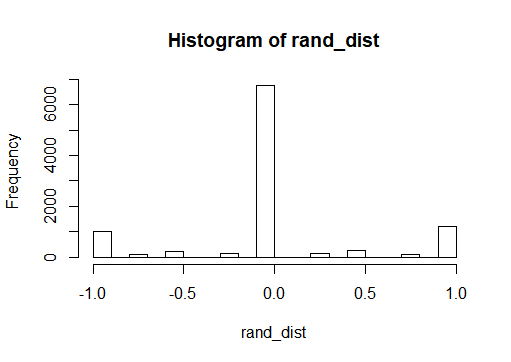
\includegraphics[width=\linewidth]{hist.png}
	\caption{Histogram.}
	\label{fig:hist}
\end{figure}

\begin{lstlisting}[language=R]
	#b) Xac suat de dien tich hinh vuong khong qua 0.5 m2
	X <- function(){
		x <- runif(1, min = 0, max = 1)
		return (x^2 <= 0.5)
	}
	tansuat <- function(N){
		ketqua <- replicate(N, X())
		return (sum(ketqua)/N)
	}
	
	#Test
		> tansuat(500000)
		[1] 0.707494

\end{lstlisting}

\section{Tham khảo}
\label{Tham khao}
[1] Introduction to R, \href{https://campus.datacamp.com/courses/free-introduction-to-r}{Datacamp}. \\

\end{document}